\section{Evaluation}
\label{rate-limiter:sec:evaluation} 


\begin{figure*}[!tb]
\centering

\begin{subfigure}[b]{0.45\textwidth}
\centering
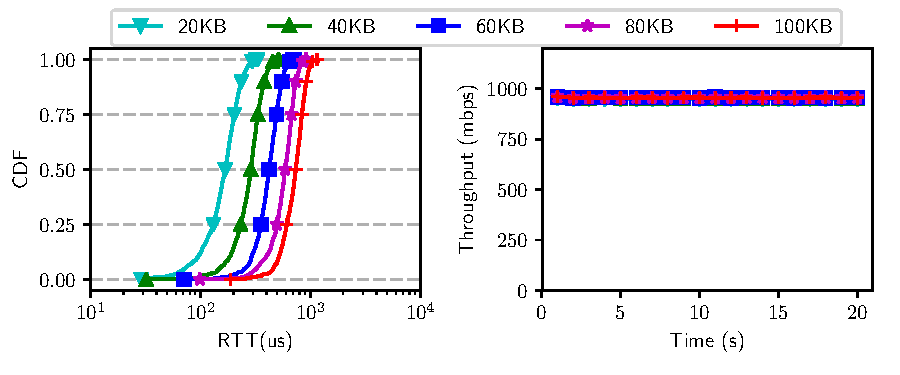
\includegraphics[width=\textwidth]{rate_limiter/raw_data/dem_benchmark/1gbps.pdf}
\caption{Rate Limiting: 1Gbps}
\label{fig:dem-1g} 
\end{subfigure}
\begin{subfigure}[b]{0.45\textwidth}
\centering
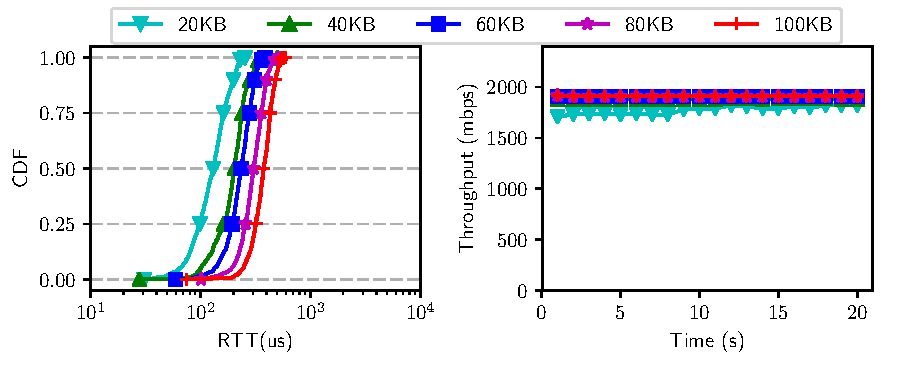
\includegraphics[width=\textwidth]{rate_limiter/raw_data/dem_benchmark/2gbps.pdf}
\caption{Rate Limiting: 2Gbps}
\label{fig:dem-2g} 
\end{subfigure}
\caption{\dem{} experiments, 1flow, varying threshold}
\label{fig:dem} 
\end{figure*}


\begin{figure*}[!t]
\centering
\begin{subfigure}[b]{0.45\textwidth}
\centering
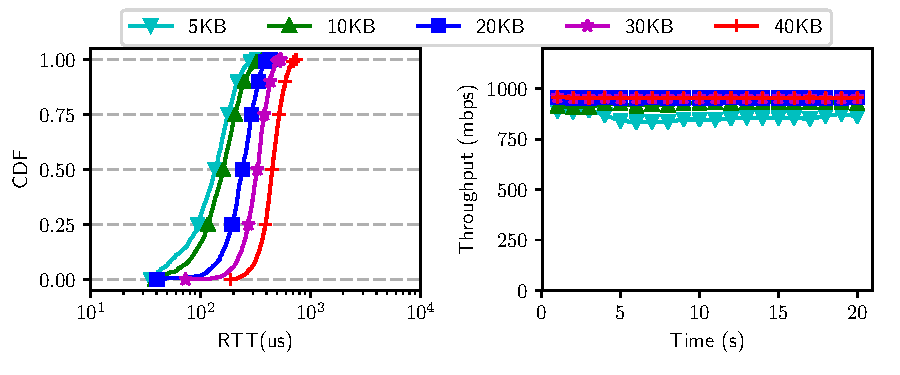
\includegraphics[width=\textwidth]{rate_limiter/raw_data/spring_benchmark/1gbps.pdf}
\caption{Rate Limiting: 1Gbps, $K2$=$K1$+10KB}
\label{fig:spring-1g} 
\end{subfigure}
\begin{subfigure}[b]{0.45\textwidth}
\centering
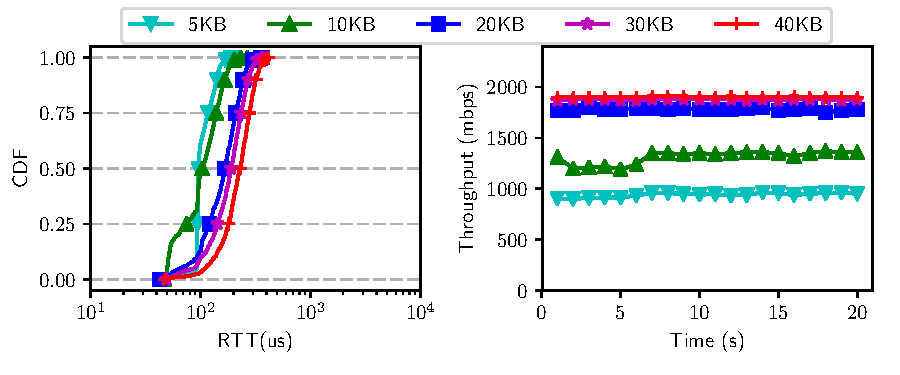
\includegraphics[width=\textwidth]{rate_limiter/raw_data/spring_benchmark/2gbps.pdf}
\caption{Rate Limiting: 2Gbps, $K2$=$K1$+20KB}
\label{fig:spring-2g} 
\end{subfigure}
\caption{\nametwo experiments, $\alpha=0.5$, $\beta=0.5$, 1 flow, varying threshold}
\label{fig:spring} 
\end{figure*}


\begin{figure}[!t]
\centering
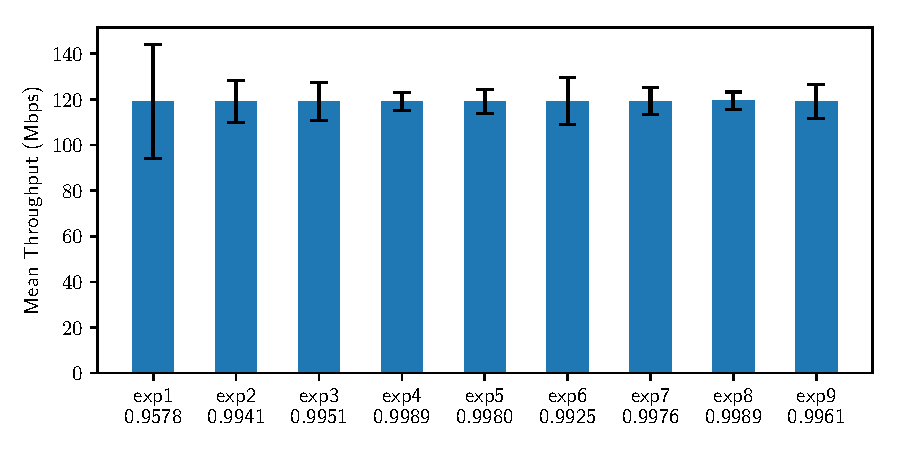
\includegraphics[width=0.5\textwidth]{rate_limiter/raw_data/spring_fairness/figure.pdf}
\caption{~\spring{} throughput fairness: 9 runs, 8 flows per run, rate-limiting=1Gbps, fairness index at the bottom}
\label{fig:spring:fairness}
\end{figure}

\begin{figure}[!t]
\centering
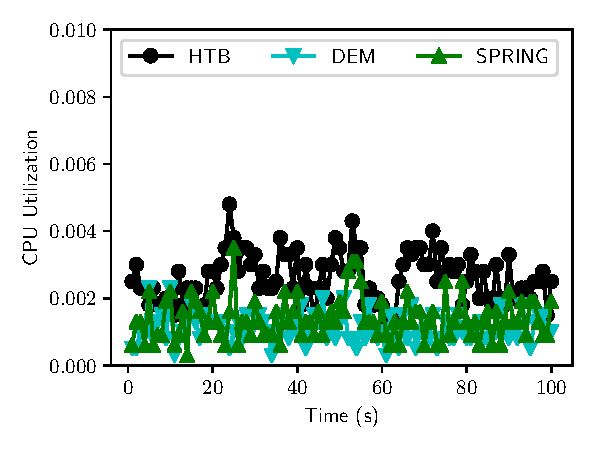
\includegraphics[width=0.5\textwidth]{rate_limiter/raw_data/cpu_overhead/figure.pdf}
\caption{CPU overhead}
\label{fig:cpu-overhead}
\end{figure}


We evaluate the performance of~\dem{} and~\spring{} in this section. 
We use CloudLab as our testbed and configure rate limiters using Linux HTB 
(Hierarchical Token Bucket). We modify OVS and HTB to implement~\dem{} and ~\spring{}. 
In the following, we will show the throughput, latency, fairness and 
CPU overhead of ~\dem{} and~\spring{} enabled rate limiters.

\tightparagraph{~\dem{} performance} 
We setup two servers. One acts as the sender and the other as the receiver. 
On the sender side, we configure rate limiter (HTB) to different speeds 
(500Mbps, 1Gbps, 2Gbps, 4Gbps, 6Gbps and 8Gbps). 
We also enable DCTCP on the two servers.~\dem{} directly sets TCP ECE bit 
if real time rate limiter queue length is above a pre-configured threshold $K$. 
For each rate limiter speed, we vary threshold $K$. 
Then we measure the throughput using iperf and TCP RTT using sockperf. 
The results are shown in Figure~\ref{fig:dem}. 
We can see that~\dem{} can greatly reduce the latency caused by rate limiters (latency is decreased by around 10 times). 
Also it gives high and stable TCP throughput (throughput is the same as raw HTB).
We also benchmark the performance of~\dem{} with multiple iperf flows and the results show similar trends.

\tightparagraph{~\spring{} performance}
We run~\spring{}-enabled rate limiters on the sender side. The rate limiter (HTB) is 
configured with different speeds (500Mbps, 1Gbps, 2Gbps, 4Gbps, 6Gbps and 8Gbps). Then we 
send an iperf flow (to measure throughput) and a sockperf flow (to measure TCP RTT). The 
experiment results for rate limiter speed of 1Gbps and 2Gbps are shown in Figure~\ref{fig:spring}. 
Similar to~\dem{}, when the algorithm parameters are appropriate,~\spring{} gives 
very stable and high throughput saturation while latency is close to the case where there is no congestion. 
We also increase the number of concurrent iperf flows and the results show similar trends.

\tightparagraph{Throughput fairness}
We run an experiment to check throughput fairness of~\spring{}. We fix the rate limiter (HTB) 
speed to 1Gbps and send 8 concurrent iperf flows through the rate limiter. 
Figure~\ref{fig:spring:fairness} shows the results. We perform the experiment for 9 runs and each run lasts 
for 20 seconds. We can see that in all runs, TCP throughput fairness index is above 0.95.

\tightparagraph{CPU overhead}
The operations of~\dem{} and~\spring{} are pretty light-weight. 
So their CPU overhead should be very small. We conduct an experiment to 
validate this---we run raw HTB,~\dem{}-enabled HTB and~\spring{}-enabled HTB and 
fix the rate limiter speed to 2Gbps. We send TCP traffic to saturate the rate limiterand and 
measure the CPU usage of sender server (the sender server has 40 cores). 
Figure~\ref{fig:cpu-overhead} shows the experiment results. 
Indeed, both~\dem{} and~\spring{} incurs very little CPU overhead and surprisingly, 
it is slightly smaller than raw HTB's. 
We think it might be caused by the fact 
that~\dem{} and~\spring{} reduce throughput slightly. 

